\section*{Question 1:}
Exercise 6.2: 

Create a simple spelling corrector based on the noisy channel model. Use a single-word language model, and an error model where all errors with the same edit distance have the same probability. Only consider edit distances of 1 or 2. Implement your own edit distance calculator (example code can easily be found on the Web).

\subsection*{Answer:}
I have used the WikiSmall collection provided on the book website as a sample:

http://www.search-engines-book.com/collections/



\pagebreak
Google found about 377,000,000 results for the term ``Memory''.
\begin{figure}[h]
\caption{Query: Memory, Search Engine: Google}
\centering
%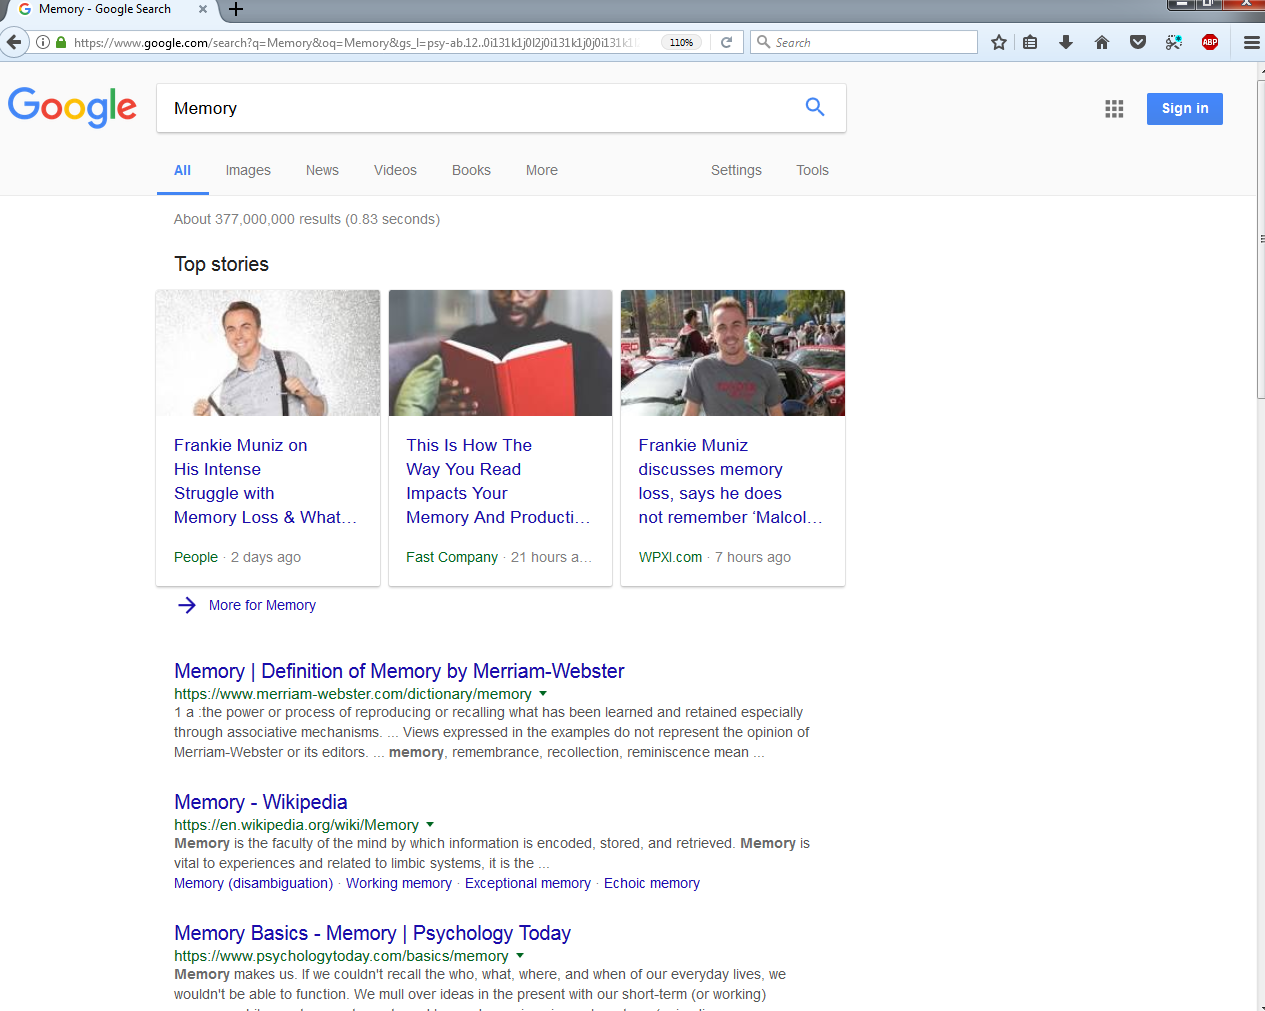
\includegraphics[scale=0.4]{Q1/MemoryGoogle.png}
\end{figure}
